% !TEX root = ./rosbook_jp.tex
%-------------------------------------------------------------------------------
\chapterimage{chapter_head_5.pdf}

%-------------------------------------------------------------------------------
\chapter{ROSツール}\index{ROSツール}

本章では、ROSを用いたプログラム開発で利用できる便利なツールを紹介する。この章で説明するツールは、次の通りである。

\begin{itemize}
\item [RViz] 3次元可視化ツール
\item [rqt] QtベースのROS GUI開発ツール
\item [rqt\_image\_view] カメラ映像を表示するツール
\item [rqt\_graph] ノードとメッセージ間の関係をグラフで表示するツール
\item [rqt\_plot] 2次元データのプロットツール
\item [rqt\_bag] GUIベースのbagデータ分析ツール
\end{itemize}

%-------------------------------------------------------------------------------
\section{3次元可視化ツール RViz}\index{3次元可視化ツール RViz}

RVizは、ROSの3次元可視化ツールである。RVizはROSネットワーク上のデータを3次元的に可視化でき、センサの計測データの確認や3次元コンピュータグラフィックスによるロボットの動作確認などに利用できる。例えば、レーザーレンジファインダー(LRF、Laser Range Finder)などの距離センサから得られる距離データ、KinectやXtionなどの3次元センサから得られる点群データ(PCD、Point Cloud Data)、カメラから取得したカラー画像などが表示できる。図5-1から図5-4は、それぞれ超音波センサ、Kinect、LRF、Xtionのデータを3次元的に可視化した例である。

RVizでは、あらかじめ用意された多くの画面設定(ディスプレイ)から適切なものを選択することで、多様な情報が表示できる。例えば、ディスプレイの一つであるInteractive Markersを使用すると、対象物の可視化と同時に、指定した対象物の位置・姿勢をユーザーが自由に変えることができ、インタラクティブなノードとユーザー間の情報(ロボットアームの位置・姿勢や目的地の位置・姿勢など)のやりとりが可能になる。また、3次元モデルの記述法であるURDF(Unified Robot Description Format)フォーマットでロボットを定義し、ファイルに保存しておけば、RVizはそのファイルを読み込み、3次元コンピュータグラフィックスでロボットを表示できる。さらに、モデルに関節自由度や移動自由度を定義しておけば、ロボットの位置や姿勢を変更でき、シミュレーションや実時間でのロボットの動作確認に利用できる。


\begin{figure}[htp]
  \centering
  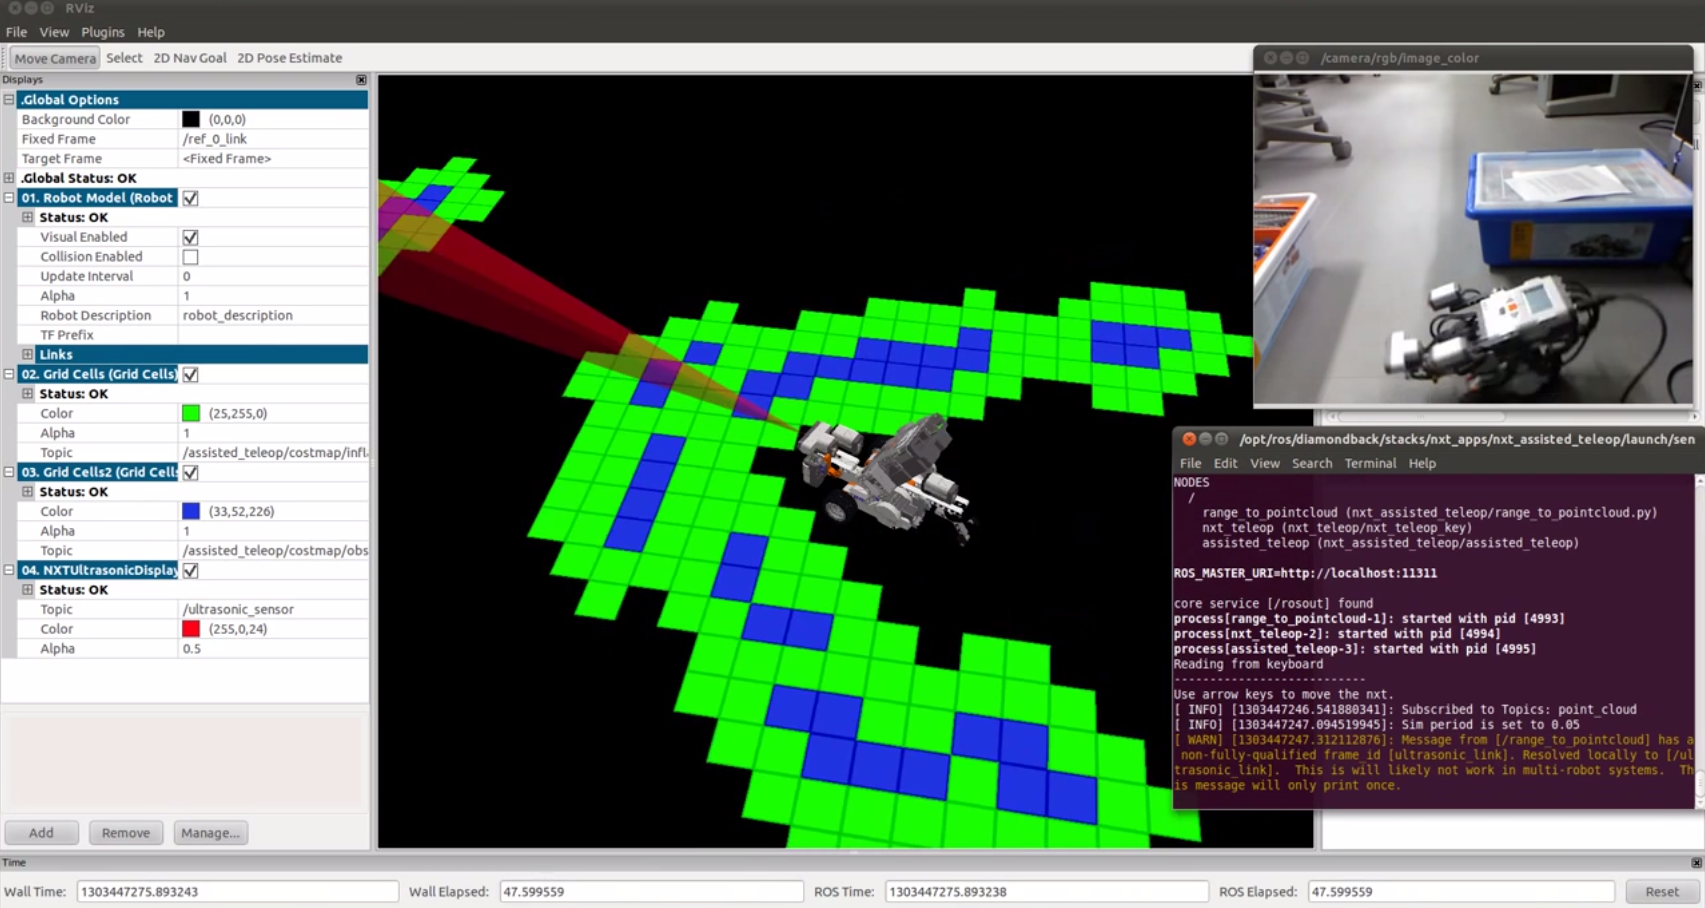
\includegraphics[width=\columnwidth]{pictures/chapter5/pic_05_01.png}
  \caption{RViz使用例1:LEGOロボットと超音波センサを用いた簡単なマップの作成の例}
\end{figure}

\begin{figure}[htp]
  \centering
  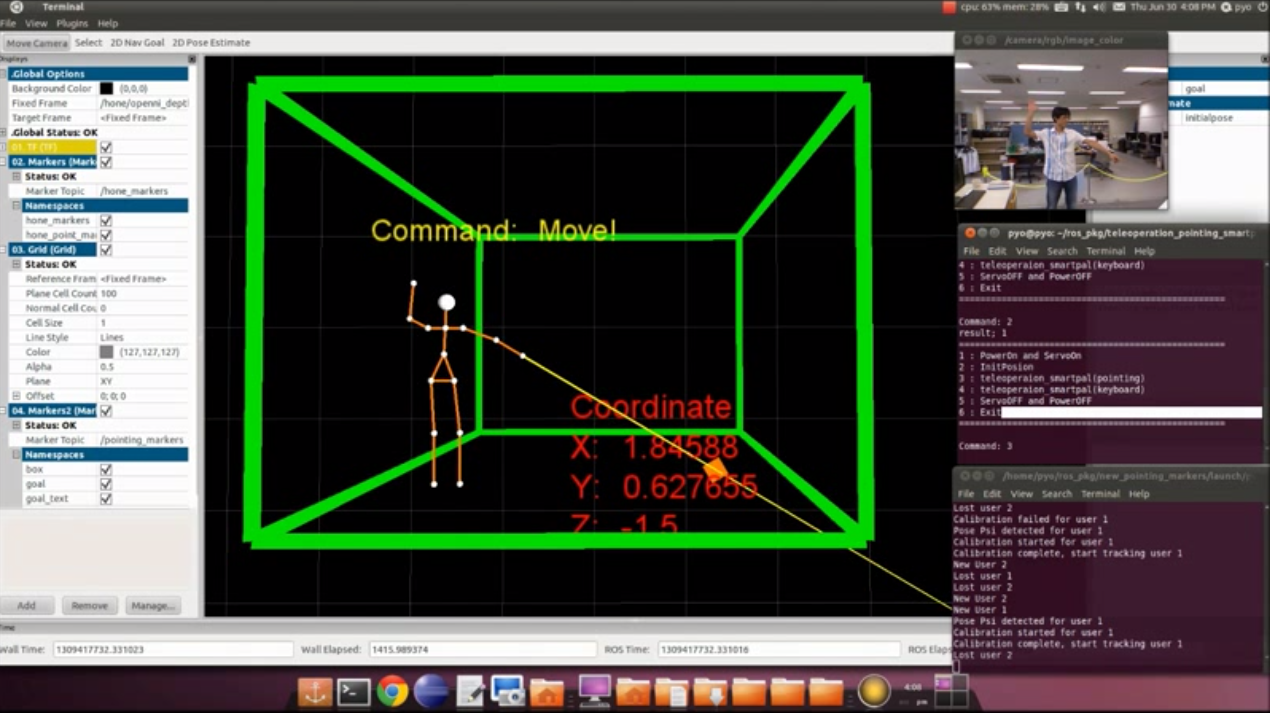
\includegraphics[width=\columnwidth]{pictures/chapter5/pic_05_02.png}
  \caption{RViz使用例2:Kinectから人の骨格を取得し、ロボットを制御している例}
\end{figure}

\begin{figure}[htp]
  \centering
  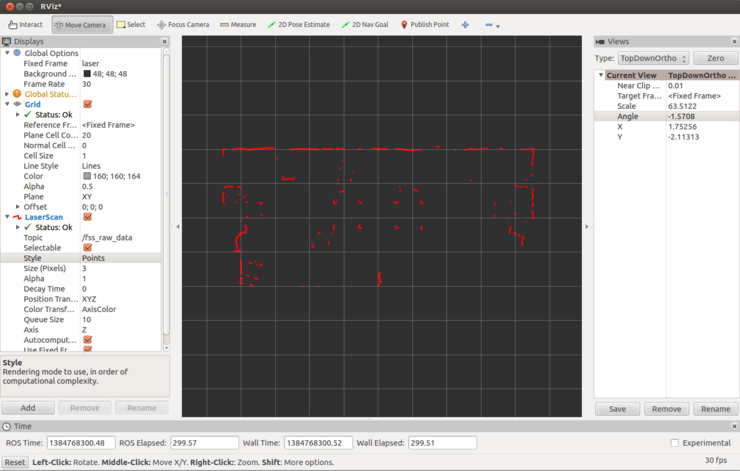
\includegraphics[width=\columnwidth]{pictures/chapter5/pic_05_03.png}
  \caption{RViz使用例3:LRFを用いた距離計測の例}
\end{figure}

\begin{figure}[htp]
  \centering
  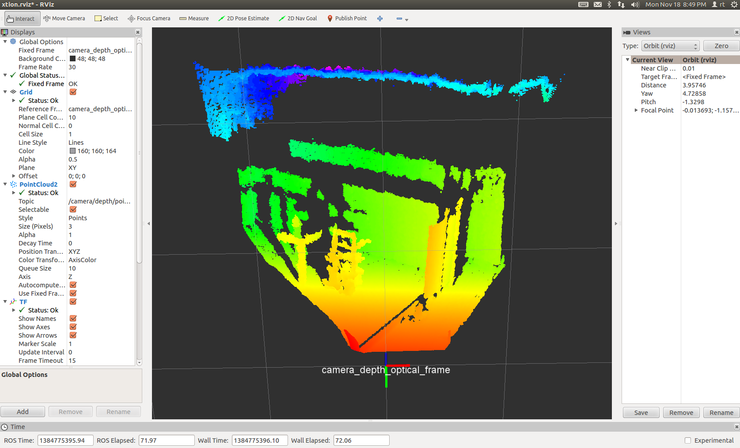
\includegraphics[width=\columnwidth]{pictures/chapter5/pic_05_04.png}
  \caption{RViz使用例4:Xtionセンサから取得した3次元距離値の例}
\end{figure}

%-------------------------------------------------------------------------------
\subsection{RVizのインストールと実行}

RVizは、ROSを第2章で紹介した方法に従い「sudo apt-get install ros-indigo-desktop-full」でインストールすると、自動的にインストールされる。もし上記以外の方法によりRVizがインストールされていない場合は、次のコマンドでインストールする。

\vspace{\baselineskip}
\begin{lstlisting}[language=ROS]
$ sudo apt-get install ros-indigo-rviz
\end{lstlisting}

RVizの実行コマンドは、次のとおりである。ただし、roscoreが実行されている必要がある。

\vspace{\baselineskip}
\begin{lstlisting}[language=ROS]
$ rosrun rviz rviz
\end{lstlisting}

%-------------------------------------------------------------------------------
\subsection{RVizの画面構成}

RVizの画面構成について、図5-5を用いて説明する。

\begin{figure}[htp]
  \centering
  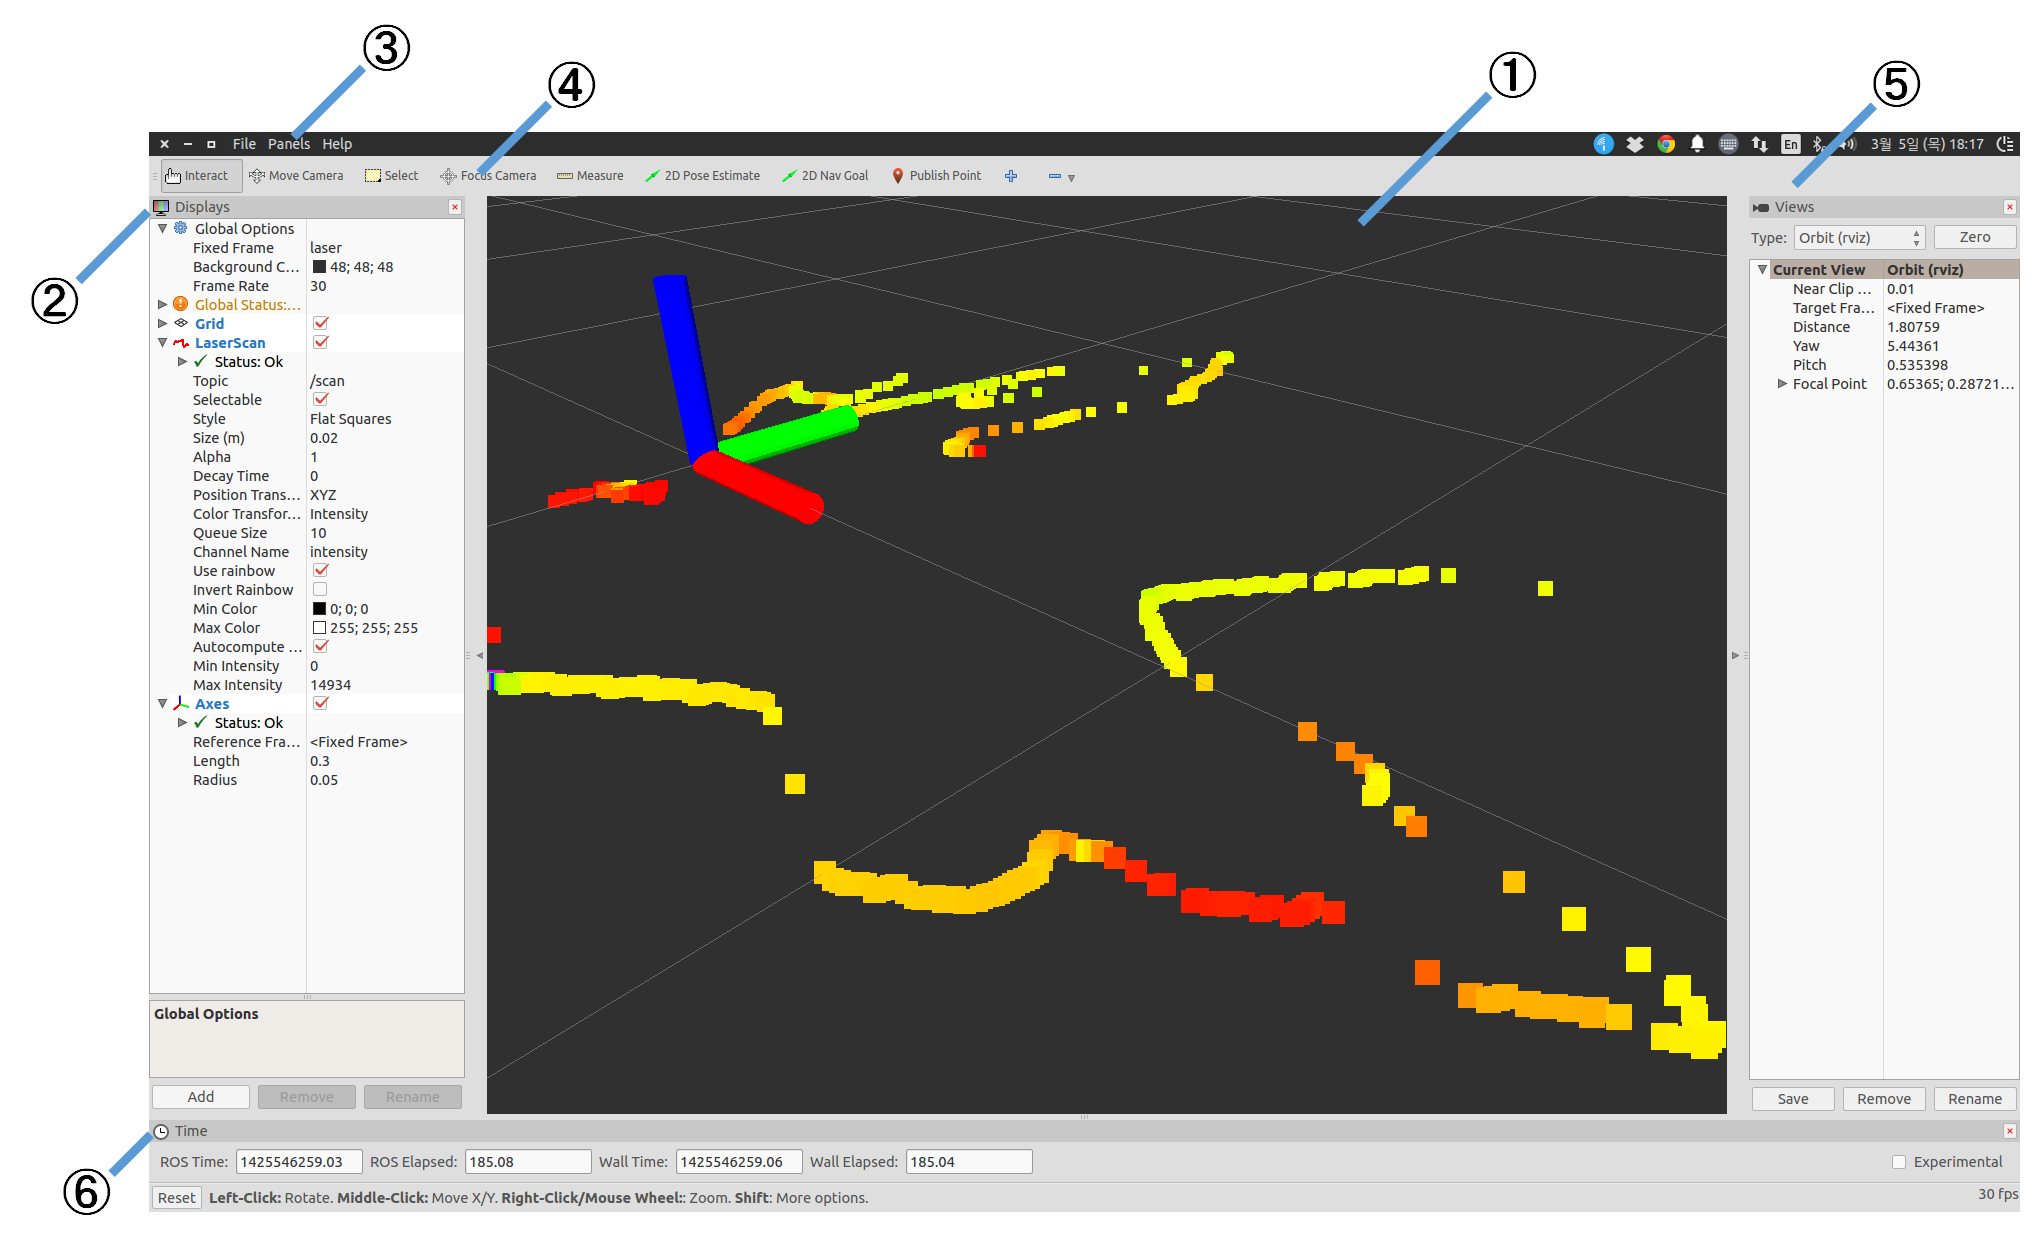
\includegraphics[width=\columnwidth]{pictures/chapter5/pic_05_05.png}
  \caption{RVizの画面構成}
\end{figure}

\begin{itemize}
\item 3Dビュー(3D view):各種データを3次元的に表示するメイン画面である。3Dビューの背景色、固定フレーム、グリッドなどは左側のディスプレイ(Displays)のGlobal OptionsとGrid項目で設定できる。
\item ディスプレイ(Displays):左側にあるディスプレイ設定画面では、様々なトピックに対して、それぞれ適切なデータの表示方法(ディスプレイ)を選択できる。ディスプレイの選択は、画面の左下の<Add>をクリックし、表示された図5-6の選択画面でおこなう。現在、約30種類のディスプレイを選択できる。これについては、後で詳しく説明する。
\itemメニュー(Menu):上部に置かれているメニューでは、現在の表示状態の保存や読み込み、各パネル(3Dビューやディスプレイ、ツールなど)の表示・非表示の切替えができる。
\item ツール(Tools):上部にあるボタンで、カメラの移動、選択、視点方向の変更、距離測定、2次元位置推定、ロボットの移動目標点、パブリッシュポイントなど、様々な機能を実行できる。パブリッシュポイントとは、3Dビュー内をマウスでクリックした点が、/clicked\_pointトピックとして配信される機能である。
\itemビュー(Views):3Dビューの視点を設定する。
  \begin{itemize}
  \item Orbit:特定の3次元位置(注視点)を中心に視点を回転する。(規定値)
  \item FPS(first-person):現在の視点位置を中心に視点を回転する。
  \item TopDownOrtho:XY平面を上からみた視点である。他のビューとは異なり、透視投影法ではなく、平行投影法で表示する。
  \item  XYOrbit:規定値であるOrbitと似ているが、注視点がXY平面上に固定されている。
  \end{itemize}
\item 時間(Time):現在の時間(wall time)とROS Time、またそれぞれの経過時間を示す。経過時間を再起動するには、一番下の<Reset>ボタンをクリックする。
\end{itemize}

\begin{figure}[htp]
  \centering
  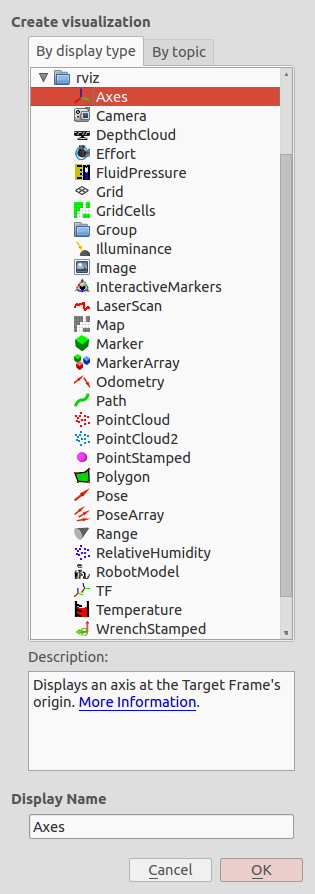
\includegraphics[width=\columnwidth]{pictures/chapter5/pic_05_06.png}
  \caption{RVizディスプレイの選択画面}
\end{figure}

表5-1 Rvizディスプレイ

アイコン  名前  説明

\begin{description}
\item  [Axes]  xyz軸を表示する。
\item  [Camera]  カメラの視点から、新しいレンダリングウィンドウを表示し、その上に画像をオーバーレイする。
\item  [DepthCloud]  奥行き地図(depth map)から得られる点群ポイントクラウド(point cloud)を表示する。主にKinect、Xtionなどのセンサの距離画像(DepthMapトピック)に、カメラ画像(ColorImageトピック)を付加した、色情報の付いた点群データで表示する。
\item  [Effort]  ロボットの各回転関節の力を表示する。
\item  [FluidPressure] 空気、水のような流体の圧力を表示する。
\item  [Grid]  2次元または3次元のグリッドを表示する
\item  [Grid Cells]  グリッドの各セルを表示する。主にナビゲーションのcostmapの障害物表示に使用される。
\item  [Group] ディスプレイをグループ化するコンテナである。ディスプレイを1つのグループとして管理できる。
\item  [Illuminance] 照度を表示する。
\item  [Image] 画像を新しいレンダリングウィンドウに表示する。Cameraディスプレイとは異なり、カメラオーバーレイはしない。
\item  [InteractiveMarkers]  単一または複数のInteractive Markerを表示する。Interactive Markerは、マウスで位置(x、y、z)と姿勢(roll、pitch、yaw)を変えることができる。
\item  [LaserScan] レーザースキャン値を表示する。
\item  [Map] ナビゲーションで使用する占有地図(occupancy map)をground plane上に表示する。
\item  [Marker]  RVizで提供される矢印、円、三角形、長方形、シリンダなどのマーカーを表示する。
\item  [MarkerArray] 上記マーカーを複数表示する。
\item  [Odometry]  時間の経過に伴うオドメトリ(odometry)情報を矢印で表示する。例えば、ロボットが移動すると、通り過ぎたパス上に、矢印マーカーが一定の時間間隔で表示される。
\item  [Path]  ナビゲーションで使用されるロボットの経路を表示する。
\item  [Point Cloud] ポイントクラウド(point cloud)のデータを表示する。Kinect、Xtionなどの3次元計測器から得られる点群データを表示するために使用する。PointCloudとPointCloud2の2種類の形式があり、PointCloud2が最新のPCL(Point Cloud Library) 注1で使用しているフォーマットである。一般的にはPointCloud2を使用すればよい。
\item  [Point Cloud2]
\item  [PointStamped]  丸いポイントを表示する。
\item  [Polygon] ポリゴン(polygon)のアウトラインを表示する。主にロボットの外形などを簡単に2次元上に表現するために使用される。
\item  [Pose]  2次元上のpose(位置と姿勢)を表示する。 Poseを矢印で表現する時、矢印の原点は位置(x、y)を表し、矢印の方向は姿勢(yaw)を示す。ロボットの位置と姿勢や、ナビゲーションの目的点(goal point)にも使用される。
\item  [Pose Array]  上記のposeを複数表示する。
\item  [Range] 超音波や赤外線センサなどの距離センサの測定範囲を円錐形で可視化する。
\item  [RelativeHumidity] 相対湿度を表示する。
\item  [RobotModel]  ロボットモデルを表示する。
\item  [TF]  座標変換値であるtfを表示する。
\item  [Temperature] 温度を表示する。
\item  [WrenchStamped] 「矢印」(力)と「矢印+丸」(トルク)でねじり動作であるレンチ(wrench)を表示する。
\end{description}

%-------------------------------------------------------------------------------
\section{ROS GUI開発ツール rqt}\index{ROS GUI開発ツール rqt}

ROSには、3D視覚化ツールであるRViz以外にも、ロボットの開発に必要な様々なGUIツールがある。例えば、各ノードの階層構造をグラフで示し、現在のノードとトピックの状態を確認できるツールや、トピックのデータを2次元プロットで図示するツールなどである。
ROS Fuerteバージョンから、RVizを含むこれら30種類以上のGUIツールがrqtという名前で統合されて、総合GUIツールとして使用できるようになった。さらに、rqtはその名前が示すようにQtで開発されており、ユーザーが自由にプラグインを開発し追加できる。この節では、rqtのインストール方法から一般的な使い方、さらにrqtのプラグインでも特に使用頻度の高いrqt\_image\_view、rqt\_graph、rqt\_plot、rqt\_bagについて述べていく。

%-------------------------------------------------------------------------------
\subsection{rqtのインストール}

rqtは、ROSを第2章で紹介した方法に従い「sudo apt-get install ros-indigo-desktop-full」でインストールすると、自動的にインストールされる。もし上記以外の方法によりrqtがインストールされていない場合は、次のコマンドでrqtをインストールする。

\vspace{\baselineskip}
\begin{lstlisting}[language=ROS]
$ sudo apt-get install ros-indigo-rqt ros-indigo-rqt-common-plugins
\end{lstlisting}

ただし、rqt\_plotでは、グラフ作成のために追加でインストールしなければならないファイルがある。rqt\_plotはPyQtGraph、MatPlot、QwtPlotをサポートしているが、ここではPyQtGraphを使用する。次のアドレスから最新のpython-pyqtgraph\_0.9.xx-x\_all.debファイルをダウンロードし、インストールする。

http://www.pyqtgraph.org/downloads/

インストールが完了したら、次のコマンドでrqt\_plotを実行する。

\vspace{\baselineskip}
\begin{lstlisting}[language=ROS]
$ rqt_plot
\end{lstlisting}

rqt\_plotを実行し、右上隅にある歯車の形のアイコン(オプションを意味する)をクリックする。表示された図5-7のオプション選択画面で、「Plot Type」の中から「PyQtGraph」を選択する。

\begin{figure}[htp]
  \centering
  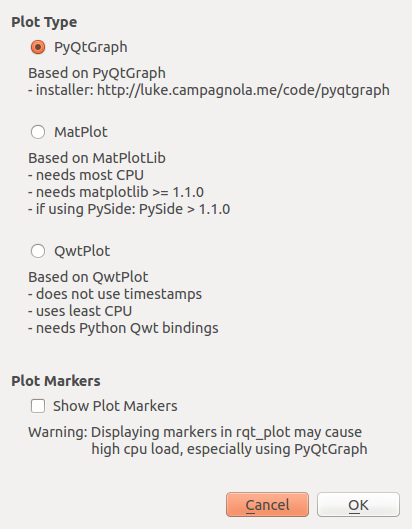
\includegraphics[width=\columnwidth]{pictures/chapter5/pic_05_07.png}
  \caption{rqt\_plotのオプション選択画面}
\end{figure}

%-------------------------------------------------------------------------------
\subsection{rqtの実行とメニュー}

rqtを実行するコマンドは次のとおりである。単にrqtと入力するか、「rosrun rqt\_gui rqt\_gui」と入力する。

\begin{lstlisting}[language=ROS]
$ rqt
\end{lstlisting}

rqtを実行すると、図5-8のようにrqtのgui画面が現れる。初めて起動したときには、メニューのみが表示される。これは、rqt上で実行するプラグインが指定されていないためである。

\begin{figure}[htp]
  \centering
  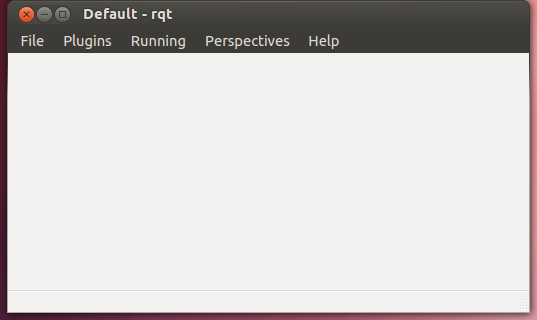
\includegraphics[width=\columnwidth]{pictures/chapter5/pic_05_08.png}
  \caption{rqtの初期画面}
\end{figure}

rqtの各メニューは、次のとおりである。

\begin{itemize}
\item ファイル(File):rqtを終了するサブメニューがある。
\item プラグイン(Plugins):30種類以上のプラグインがある。これらを選択して使用する。
\item 動作(Running):現在動作中のプラグインを表示し、不要なプラグインを停止できる。
\item 画面構成(Perspectives):現在動作中のプラグインを保存し、次回の起動時に同じプラグインを実行できる。
\end{itemize}

%-------------------------------------------------------------------------------
\subsection{rqtプラグイン}

rqtの上部メニューの中から[プラグイン(Plugins)]を選択すると、30種類以上のプラグインが以下の項目に分類されて表示される。ここではrqtの基本的なプラグインを紹介するが、必要なら非公認のrqtプラグインや、ユーザーが開発したrqtプラグインも追加できる。

\textbf{アクション(Action)}
\begin{description}
\item  [Action Type Browser] Actionタイプのデータ構造を確認する。
\end{description}

\textbf{構成(Configuration)}
\begin{description}
\item  [Dynamic Reconfigure] ノードのパラメータ値を変更できる。
\item  [Launch] roslaunchのGUIプラグイン。roslaunchの名前や構成が思い出せないときに便利である。
\end{description}

\textbf{内部構造(Introspection)}
\begin{description}
\item  [Node Graph] 実行されているノードの関係図やメッセージの流れをグラフビュー形式で確認できる。
\item  [Package Graph] パッケージの依存関係をグラフビュー形式で表示する。
\item  [Process Monitor] 現在実行中のノードのPID(プロセッサID)、CPU使用率、メモリ使用率、スレッドの数を確認できる。
\end{description}

\textbf{ロギング(Logging)}
\begin{description}
\item  [Bag] ROSデータロギング関連のプラグイン
\item  [Console] ノードで発生する警告(Warning)、エラー(Error)などのメッセージを一つの画面で確認できる。
\item  [Logger Level] ノードでログ発行を担当するロガーを選択し、ロガーレベルと呼ばれるDebug、Info、Warn、Error、Fatalログ情報を設定するためのプラグイン。デバッグするときDebugを選択して使用すると、非常に便利である。
\end{description}

\textbf{様々なツール(Miscellaneous Tools)}
\begin{description}
\item  [Python Console] Pythonのコンソール画面のプラグイン
\item  [Shell] シェルを駆動する。
\item  [Web] ブラウザを駆動する。
\end{description}

\textbf{ロボット(Robot)}
\begin{itemize}
\item 使用しているロボットに応じて、ダッシュボード(dashboard)などのプラグインをここに追加すればよい。
\end{itemize}

\textbf{ロボットツール(Robot Tools)}
\begin{description}
\item  [Controller Manager] ロボットコントローラの状態、タイプ、ハードウェアインタフェース情報などを確認できる。
\item  [Diagnostic Viewer] ロボット機器およびエラーチェックを行う。
\item  [Moveit!Monitor] モーションプランニングに使用されるMoveIt!データを確認する。
\item  [Robot Steering] ロボットの手動制御GUIツール。遠隔操作では、このGUIツールを利用してロボットを操縦する。
\item  [Runtime Monitor] ノードで発生する警告やエラーを確認できる。
\end{description}

\textbf{サービス(Services)}
\begin{description}
\item  [Service Caller] 起動しているサービスサーバに接続し、サービスリクエストが可能なGUIプラグイン。サービスのテストに適している。
\item  [Service Type Browser] サービスタイプのデータ構造を確認する。
\end{description}

\textbf{トピックス(Topics)}
\begin{description}
\item  [Easy Message Publisher] GUI環境でトピックを発行するプラグインである。現在実行中のノードで使用しているトピックの中から一つのトピックを選択し、メッセージのデータをスライド・バーなどで変更しながらトピックを発行できる。これはトピックのテストに適している。
\item  [Message Publisher] Easy Message Publisherでは、選択した一つのトピックに対してメッセージの変更や配信を行うが、これは全てのトピックに対してメッセージの変更やトピックの配信ができる。トピックの内容は手動で設定する。
\item  [Message Type Browser] トピックのメッセージの型を確認する。
\item  [Topic Monitor] 現在使用しているトピックの一覧を表示し、その中でユーザーが選択したトピックの情報を表示する。
\end{description}

\textbf{可視化(Visualization)}
\begin{description}
\item  [Image View] カメラの映像データを確認できる。
\item  [Navigation Viewer] ナビゲーションで、ロボットの位置や目標地点を確認する。
\item  [Plot] 2次元データのプロットGUIプラグイン。 2次元データの可視化に非常に便利である。
\item  [Pose View] ロボットモデルやtfなどのポーズ(位置と姿勢)を表示する。
\item  [RViz] 3次元可視化ツールであるRVizのプラグイン。rqtでこれを選択すれば、RVizを起動できる。
\item  [TF Tree] tfの関係をツリー構造で表すグラフビュー形式のプラグイン
\end{description}

\begin{figure}[htp]
  \centering
  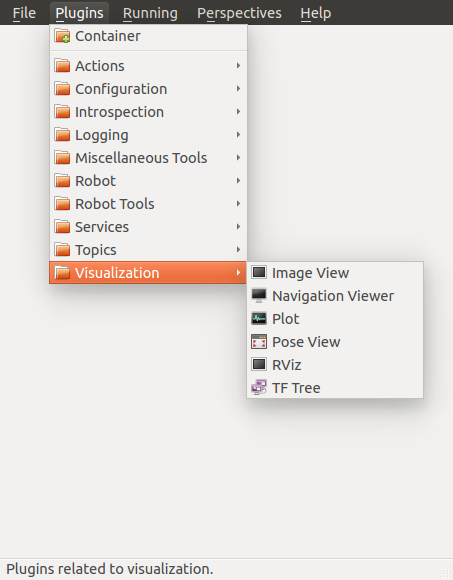
\includegraphics[width=\columnwidth]{pictures/chapter5/pic_05_09.png}
  \caption{rqtプラグイン}
\end{figure}

以降では、最も頻繁に使用されるrqt\_image\_view、rqt\_graph、rqt\_plot、rqt\_bagについて説明する。

%-------------------------------------------------------------------------------
\subsection{rqt\_image\_view}

カメラの画像データを表示するプラグインである。画像処理はできないが、取得映像を確認する用途でよく使われる。一般的なUSBカメラはUVC(USB video device class)をサポートしているので、ROSのuvc\_cameraパッケージを利用すれば簡単に画像を取得できる。まず、次のコマンドでuvc\_cameraパッケージをインストールする。

\begin{lstlisting}[language=ROS]
$ sudo apt-get install ros-indigo-uvc-camera
\end{lstlisting}

USBカメラをコンピュータのUSBに接続して、次のコマンドでuvc\_cameraパッケージのuvc\_camera\_nodeノードを実行する。

\begin{lstlisting}[language=ROS]
$ rosrun uvc_camera uvc_camera_node
\end{lstlisting}

次に「rqt」コマンドでrqtを起動し、メニューから[Plugins]→[Visualization] →[Image View]を選択する。そして、左上のトピック選択ボックスで「/image\_raw」を選択すると、図5-10のようにカメラ映像を確認できる。カメラに関しては8.1節で詳しく説明する。

\begin{lstlisting}[language=ROS]
$ rqt
\end{lstlisting}

\begin{figure}[htp]
  \centering
  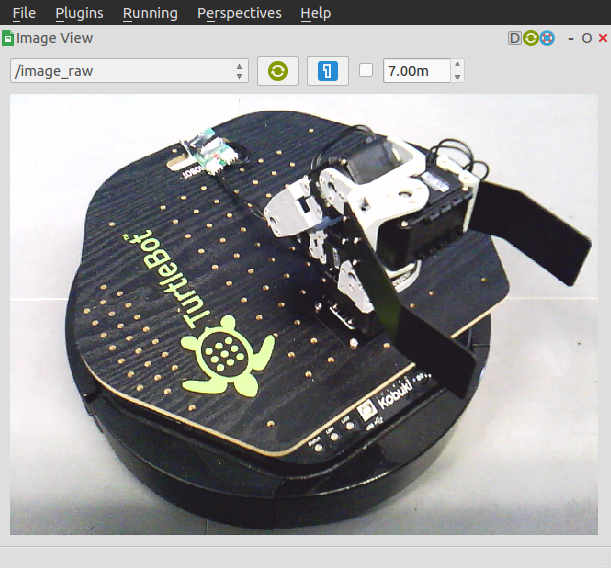
\includegraphics[width=\columnwidth]{pictures/chapter5/pic_05_10.png}
  \caption{USBカメラの画像データをrqt\_image\_viewで確認している例}
\end{figure}


%-------------------------------------------------------------------------------
\subsection{rqt\_graph}

rqt\_graphは、実行中のノードとROSネットワーク上で送受信されているメッセージの関係をグラフで表すプラグインである。ROSネットワークの状況を把握するのに非常に便利である。
ここでは、2.5節で説明したturtlesimパッケージのturtlesim\_node、turtle\_teleop\_key、そして前述のuvc\_cameraパッケージのuvc\_camera\_nodeノードを使ってrqt\_graphの使用方法を説明する。まず以下のコマンドで、関連するノードをそれぞれ別のターミナルウィンドウで立ち上げる。

\begin{lstlisting}[language=ROS]
$ rosrun turtlesim turtlesim_node
$ rosrun turtlesim turtle_teleop_key
$ rosrun uvc_camera uvc_camera_node
\end{lstlisting}

その後、次のように、「rqt」コマンドでrqtを実行して、メニューから[Plugins]→[Introspection]→ [Node\_Graph]を選択する。rqt\_graphを実行したときのノードとトピックの関係は、図5-11のように表示される。

\begin{lstlisting}[language=ROS]
$ rqt
\end{lstlisting}

\begin{figure}[htp]
  \centering
  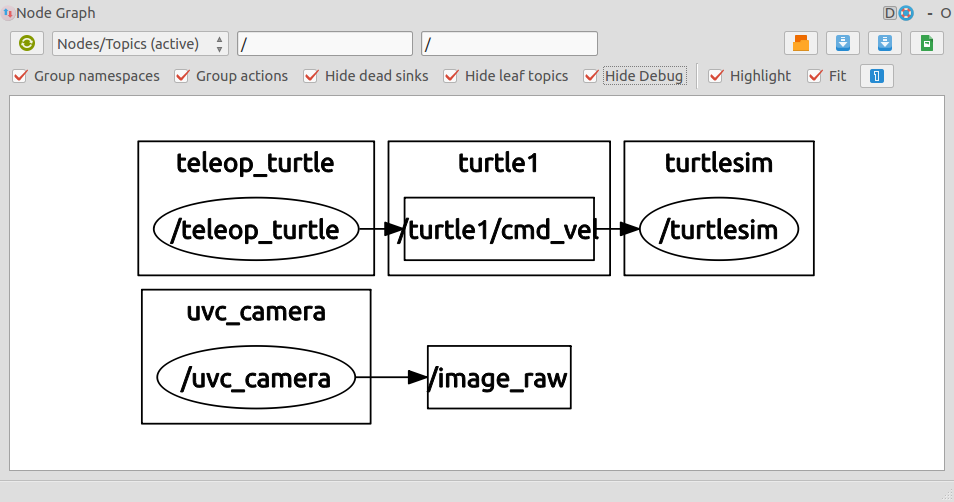
\includegraphics[width=\columnwidth]{pictures/chapter5/pic_05_11.png}
  \caption{rqt\_graph実行例}
\end{figure}

図5-11で「teleop\_turtle」などの外側の四角は名前空間のグループ(「6.5 roslaunchを用いた複数ノードの起動」を参照)を意味し、その中の「/teleop\_turtle」などの円は、実行した配信者(publisher)や購読者(subscriber)のノードを意味する。「/turtle1/cmd\_vel」と「/image\_raw」を囲む小さな四角はトピックを意味する。矢印は、トピック通信の送受信方向を意味する。図5-11の例では、turtle\_teleop\_key、turtlesim\_nodeを実行すると、teleop\_turtleとturtlesimのノードが立ち上がる。この2つのノードは、キーボードの方向キーが押されたときに配信される「/turtle1/cmd\_vel」トピックを介し、配信者と購読者の間でデータを送受信していることが確認できる。uvc\_cameraパッケージも同様に、配信者であるuvc\_cameraノードが「/imge\_raw」トピックを発行していることが確認できる。
この例ではノードを数個実行しただけであるが、実際のROSプログラミングでは、数十個に及ぶノードが様々なトピックのメッセージを送受信することも珍しくない。このようなとき、rqt\_graphは現在のROSネットワーク上のノードの関係を確認できる、非常に強力なツールである。

%-------------------------------------------------------------------------------
\subsection{rqt\_plot}

rqt\_plotは、ROSメッセージである2次元データを受け取り、2次元座標系上に描画するツールである。例として、turtlesimノードのposeメッセージのxとy座標を描画してみよう。まず、turtlesimパッケージのturtlesim\_nodeを実行する。

\begin{lstlisting}[language=ROS]
$ rosrun turtlesim turtlesim_node
\end{lstlisting}

そして、次の例のようにrqtを実行した後、メニューから[Plugins]→[Visualization]→[Plot]を選択すると、rqt\_plotが実行される。 rqt\_plot上部のTopic欄に「/turtle1/pose」と入力すれば、「/turtle1/pose」トピックが2次元(x軸:データの値、y軸:時間)の上に図式化される。

\begin{lstlisting}[language=ROS]
$ rqt
\end{lstlisting}

あるいは、次のコマンドのように、トピックを指定して実行することもできる。

\begin{lstlisting}[language=ROS]
$ rqt_plot /turtle1/pose/
\end{lstlisting}

次に、turtlesimパッケージのturtle\_teleop\_keyを実行して、画面の中の亀を前後に動かしてみよう。

\begin{lstlisting}[language=ROS]
$ rosrun turtlesim turtle_teleop_key
\end{lstlisting}

その結果、図5-12のように亀の位置、姿勢、そして速度と角速度が表示されることが確認できる。
このようにrqt\_plotは2次元データの表示に便利なツールである。今回はturtlesimに対して利用したが、ユーザーが開発したノードの2次元データの表示にも利用できる。特に、速度や加速度などの時間経過を伴うセンサの値を表示するのに適している。

\begin{figure}[htp]
  \centering
  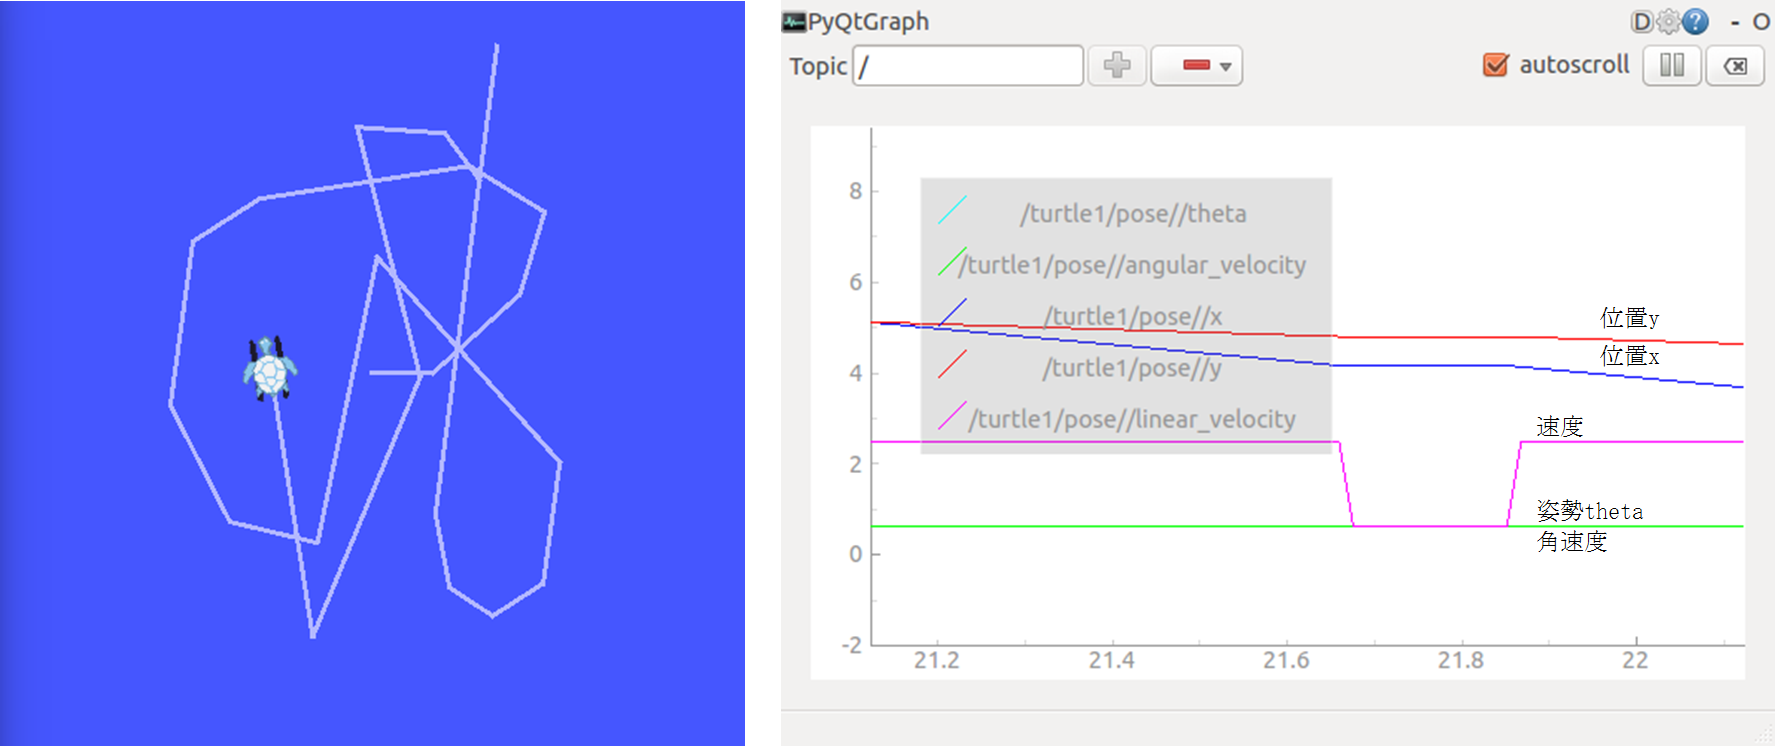
\includegraphics[width=\columnwidth]{pictures/chapter5/pic_05_12.png}
  \caption{rqt\_plotの使用例}
\end{figure}

%-------------------------------------------------------------------------------
\subsection{rqt\_bag}

rqt\_bagはbagファイルに保存したメッセージを視覚化するGUIツールである。4.4.8項で取り上げたrosbagはテキストベースであるが、rqt\_bagはこれに可視化機能が追加されたものであり、カメラ画像なども確認できる。これをテストする前に、rqt\_image\_viewと、rqt\_graphツールの説明で用いたturtlesimとuvc\_camera関連ノードをすべて実行する。次に、以下のコマンドで、uvc\_cameraの「/image\_raw」トピックとturtlesimの「/turtle1/cmd\_vel」トピックをbagファイルに保存する。

\begin{lstlisting}[language=ROS]
$ rosrun uvc_camera uvc_camera_node
$ rosbag record /image_raw
$ rqt
\end{lstlisting}

rqt\_bagは、rosbagと同様に、トピックメッセージの保存、再生、圧縮などが可能である。加えて、GUIプログラムで構成されており、すべてのコマンドはボタンで動作する。このため、操作が容易で、カメラの映像をビデオ編集プログラムのように時間軸を合わせながら確認できる。実際に、USBカメラの映像をbagファイルとして保存した後、rqt\_bagで再生してみよう。
「rqt」コマンドでrqtを実行し、メニューの[Plugins]→[Logging]→[Bag]を選択する。次に、左上のフォルダの形(Load Bag)のアイコンを選択して、上の「rosbag record /image\_raw」コマンドで記録した「*.bag」ファイルを開く。これにより、図5-13のようにカメラの映像を時間軸の変化とともに確認できる。また、このツールは映像の拡大、一定時間のデータ数の確認などができ、さらにマウスの右ボタンを押した後、「Publish」オプションをクリックすると、メッセージの再発行も可能である。

\begin{figure}[htp]
  \centering
  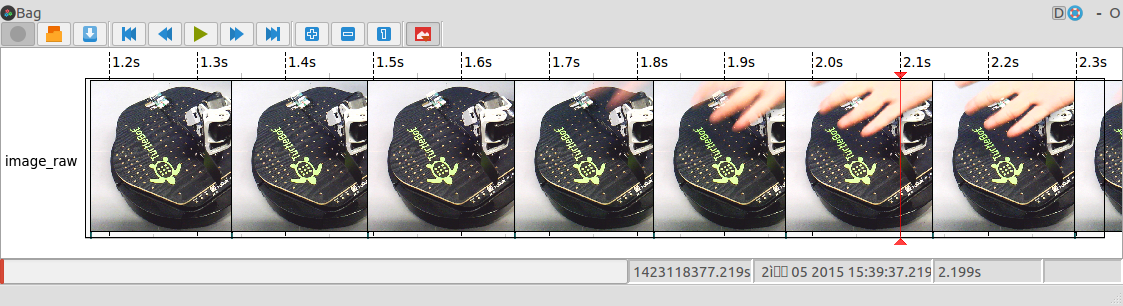
\includegraphics[width=\columnwidth]{pictures/chapter5/pic_05_13.png}
  \caption{rqt\_bagの使用例}
\end{figure}

以上でrqtツールのインストール、使用方法について概略を説明した。この節では、すべてのプラグインについては説明できなかったが、ここで示したいくつかの例を参考に、様々なオプション機能を試してほしい。rqtツールは、他のROSノードのようにロボットやセンサを直接処理するものではないが、開発作業を行う上で、データの保存、修正、分析、デバッグなどに役立つ便利な補助ツールである。

% 注1  http://pointclouds.org/
